\documentclass[a4paper]{paper}

% Set margins
\usepackage[hmargin=2cm, vmargin=2cm]{geometry}

\frenchspacing

% Language packages
\usepackage[utf8]{inputenc}
\usepackage[T1]{fontenc}
\usepackage[magyar]{babel}

% AMS
\usepackage{amssymb,amsmath}

% Graphic packages
\usepackage{graphicx}

% Colors
\usepackage{color}
\usepackage[usenames,dvipsnames]{xcolor}

% Enumeration
\usepackage{enumitem}

\begin{document}

\begin{center}
    \Large
    \textbf{Négykerekű járművek navigációs problémáinak megoldása}
   
    \medskip   
   
    \Large
    Tóth Péter
\end{center}

\vskip 1cm

\pagestyle{empty}

\section{A megoldandó probléma}

Négykerekű járművek navigálási problémáinak részletes leírása. Feltételezzük, hogy a térkép felülnézetből ismert. Az optimalizálás célja azon navigációs műveleteknek a meghatározása, amely segítségével a jármű adott pozícióból a térkép járható területein keresztül el tud jutni a célként megadott pozícióba. Fel kell írni az optimalizálási feladatokat különböző célfüggvények figyelembevételével. Meg kell jeleníteni az algoritmus által adott útvonalakat. Az optimalizálási probléma megoldása Python programozási nyelven történik a NumPy függvénykönyvtár felhasználásával.

\section{A jármű matematikai modellje}

A négykerekű jármű középpontjának a hátsó tengely középpontját tekintjük. Mivel a kanyarodásnál az első kerekek különböző szögeket zárnak be az első tengellyel, ezért érdemes egy képzeletbeli, az első tengely közepére eső kormányozható kereket megadni. Ennek a jármű irányával bezárt előjeles szögét jelöljük $\alpha$-val. A jármű tengelytávolságát jelöljük $w$-vel, a hátsó tengely hosszát pedig $a$-val (\ref{fig:vehicle}. ábra).

\begin{figure}[h!]
\centering
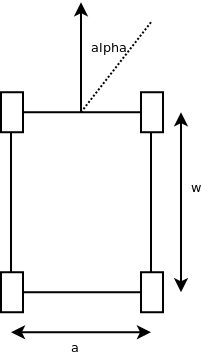
\includegraphics[scale=0.8]{images/vehicle.png}
\caption{A jármű matematikai modelljének fő paraméterei}
\label{fig:vehicle}
\end{figure}

\section{Első kerekek elfordulási szögének kiszámítása}

Az $\alpha$ szög függvényében külön ki kell számítanunk a jármű bal és jobb első kerekének elfordulási szögét.

% TODO: Részletesen leírni ezek számítását!

\section{Pozíció számítása rögzített $\alpha$ mellett}

A rögzített $\alpha$ szög, és adott sebesség mellett ki kell tudnunk számolni, hogy adott $(x_0, y_0)$ kiindulópontból indulva a jármű milyen pozícióba fog kerülni $t$ idő elteltével. Az $\alpha$ szög függvényében az alábbi módon számolhatjuk ki annak a képzeletbeli körnek a sugarát ($R$), amelyen a jármű majd kanyarodni fog:
\[
R = \dfrac{w}{\text{tg} \alpha},
\]
ahol a $w$ a jármű tengelyei közötti távolságot jelöli.

Tegyük fel, hogy a jármű sebessége $v$. Ekkor $t$ idő függvényében a jármű pozícióját az alábbi formában számolhatjuk:
\begin{align*}
x(t) &= x_0 + R - R \cdot \cos \dfrac{v \cdot t}{|R|}, \\
y(t) &= y_0 + |R| \cdot \sin \dfrac{v \cdot t}{|R|}.
\end{align*}

\end{document}
